
% \begin{figure*}[t]
%     \centering
%     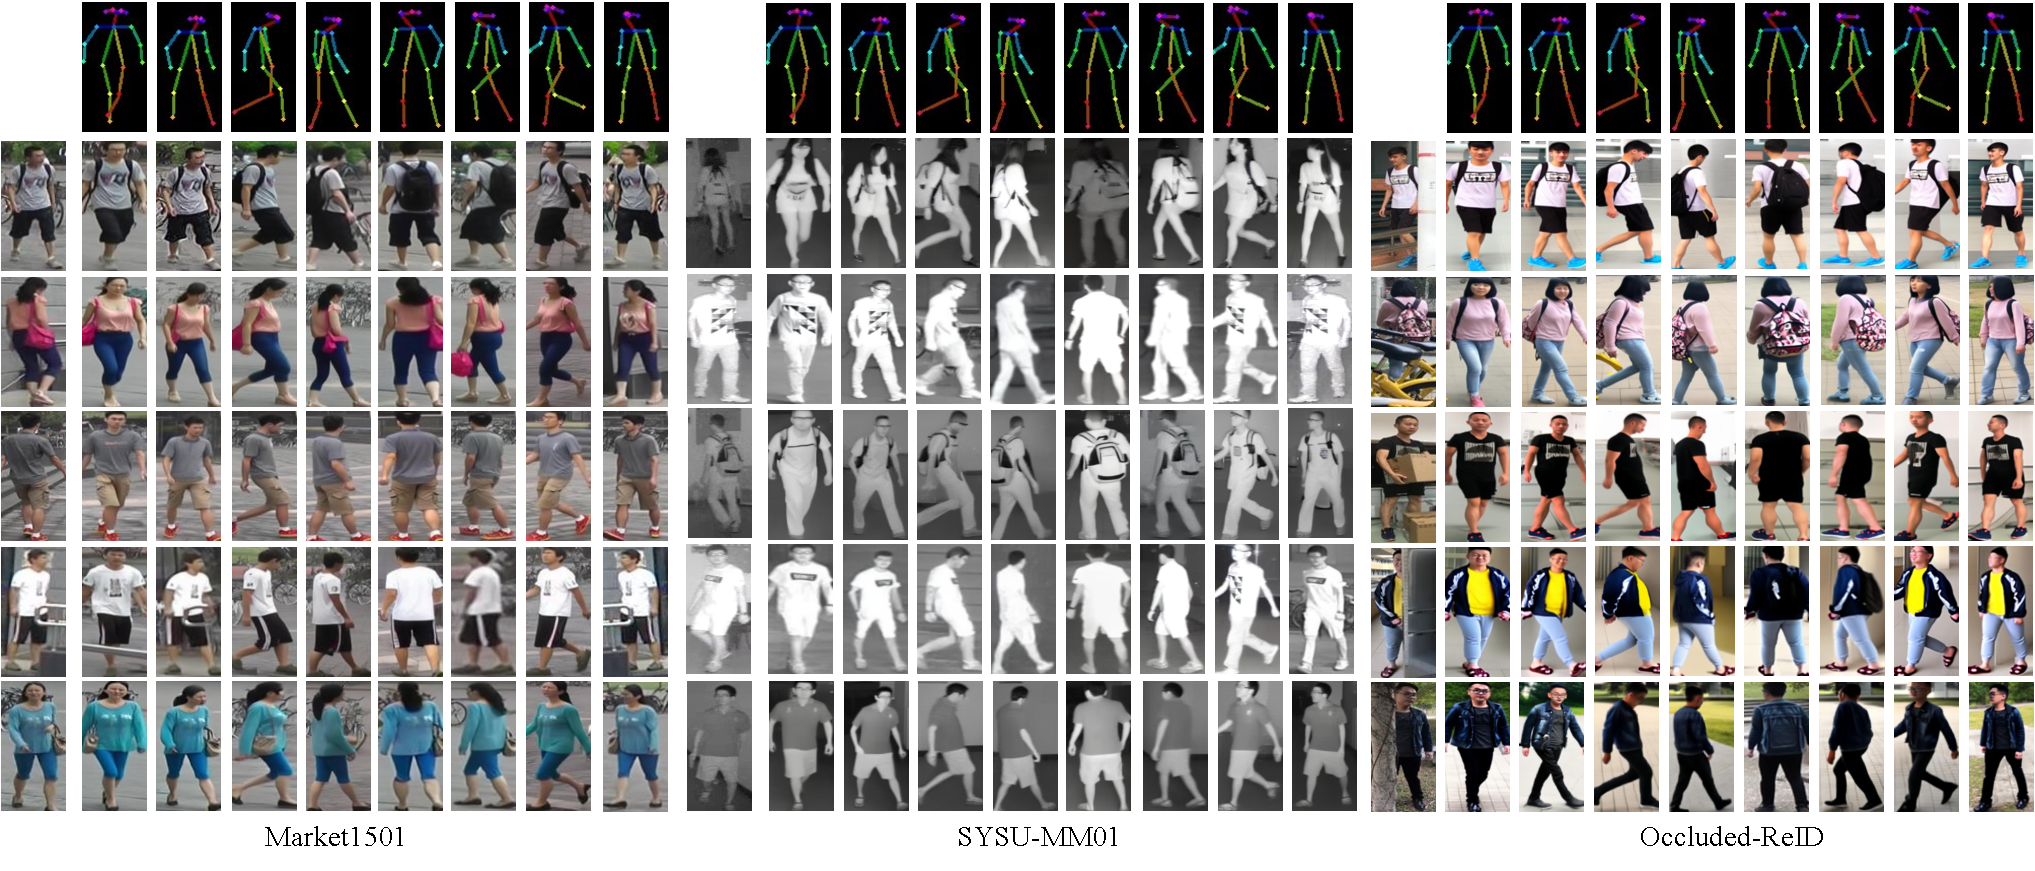
\includegraphics[width=0.9\textwidth]{figs/pdf/visualization.pdf} 
%     \label{fig:visualization}
%     \caption{Visualization of our Pedestrian Generation model with 8 directions 'standard poses' on Market1501, SYSU-MM01, and Occluded-ReID datasets.}
% \end{figure*}




\begin{abstract}
Person re-identification (ReID) aims to extract accurate identity representation features. However, during feature extraction, individual samples are inevitably affected by noise (background, occlusions, and model limitations). Considering that features from the same identity follow a normal distribution around identity centers after training, we propose a \textbf{Training-Free} \textbf{Feature Centralization} ReID framework (\textbf{Pose2ID}) by aggregating the same identity features to reduce individual noise and enhance the stability of identity representation, which preserves the feature's original distribution for following strategies such as re-ranking. Specifically, to obtain samples of the same identity, we introduce two components:
\ding{192}Identity-Guided Pedestrian Generation: by leveraging identity features to guide the generation process, we obtain high-quality images with diverse poses, ensuring identity consistency even in complex scenarios such as infrared, and occlusion.
\ding{193}Neighbor Feature Centralization: it explores each sample's potential positive samples from its neighborhood.
Experiments demonstrate that our generative model exhibits strong generalization capabilities and maintains high identity consistency. With the Feature Centralization framework, we achieve impressive performance even with an ImageNet pre-trained model without ReID training, reaching mAP/Rank-1 of 52.81/78.92 on Market1501. Moreover, our method sets new state-of-the-art results across standard, cross-modality, and occluded ReID tasks, showcasing strong adaptability.
\end{abstract}